\section{Introduction and Literature Survey}

Pinching-antenna systems (PASS) were introduced as a flexible-antenna technology in which dielectric particles are pinched onto a waveguide so that radiation can be activated at arbitrary points along the guide \cite{fukuda2022pinching}. In contrast to conventional fixed arrays, the same physical backbone can support different activation patterns without rebuilding the entire front-end. PASS therefore belongs to the broader family of flexible-antenna architectures alongside fluid antennas and movable antennas \cite{wong2021fluid,zhu2024movable,new2025tutorial,zhu2025tutorialma}, but it also has its own modeling feature: the received phasor is affected not only by the free-space propagation distance between the user and the activated antenna element, but also by a guided-wave phase term along the dielectric waveguide. This dual phase structure is precisely what makes constructive near-field focusing possible, and it is also what makes PASS unusually sensitive to position perturbations.

\subsection{Background and Motivation}

This paper brings together two active research strands. The first involves near-field and large-aperture communications, where spherical-wave propagation, location-dependent phase, and aperture geometry are the essential modeling components \cite{ouyang2024primer}. The second strand treats flexible-antenna systems, considering the geometry of radiating elements as a controllable variable \cite{wong2021fluid,zhu2024movable,new2025tutorial,zhu2025tutorialma}. The pinching-antenna-systems (PASS) framework draws on both. Prior work on PASS has shown, for example, that downlink rates improve when activated positions are chosen appropriately \cite{xu2025downlink}. The same flexibility also makes NOMA activation feasible \cite{wang2025noma} and can enforce uplink fairness constraints \cite{tegos2025uplink}. Separately, constructive alignment leads to a well-characterized nominal array gain \cite{ouyang2025array}. More recent extensions have broadened the PASS scope toward sensing \cite{ding2025isac} and tutorial-style overviews \cite{liu2026tutorial}. However, existing studies continue to emphasize nominal activation, beam/rate optimization, and the expansion of application domains. A pressing question for physical deployment remains unanswered: what are the implications when the intended pinching positions cannot be hit exactly?

This is not a trivial practical matter. In an actual PASS system, activation points are realized by pinching or displacing dielectric elements to designated spots; precise placement is difficult to guarantee.Fabrication tolerances, placement offsets, actuator limits, and calibration errors all perturb those intended positions. Once a pinching position shifts, the free-space distance changes, the waveguide path length changes, and the coherent addition of the antenna responses deteriorates. Because the PASS phase term contains the effective refractive index $n_{\mathrm{eff}}$, the sensitivity to position errors is amplified relative to purely free-space movable-antenna models. Recent movable-antenna literature has started to study the effect of position errors in near-field beamforming \cite{su2025positionerror,yang2026nearfield}, which makes the problem timely. Yet PASS deserves a dedicated treatment because its phase law is not simply geometric; it is the sum of a spherical-wave term and a guided-wave term. The resulting robustness story is therefore related to, but not identical with, the robustness story for conventional movable or fluid antennas.

Robustness also has to be decomposed carefully. A bounded independent tolerance on each activated position, a coherent common drift of the whole aperture, and a correlated displacement field do not represent the same physical failure mode and should not be expected to produce the same degradation. A useful PASS robustness study must therefore do more than attach an error bar to nominal gain. A key task is to distinguish genuinely harmful error directions from those that are primarily common-mode, and to identify conditions under which a local analytical description can still be trusted. The body of this report follows that principle: bounded adversarial errors, stochastic perturbations, and baseline comparisons are developed as related but distinct lines of evidence.

\begin{figure}[H]
\centering
\includegraphics[width=0.86\textwidth]{fig_pass_system_model_corrected.pdf}
\caption[PASS system model]{PASS system model used in this report, adapted from the array-gain formulation in \cite{ouyang2025array}. The pinching antennas are activated along a dielectric waveguide, and the received phasor combines the free-space path from each activated point to the user with the guided-wave phase accumulated along the waveguide.}
\label{fig:pass_system_model}
\end{figure}

\begin{figure}[H]
\centering
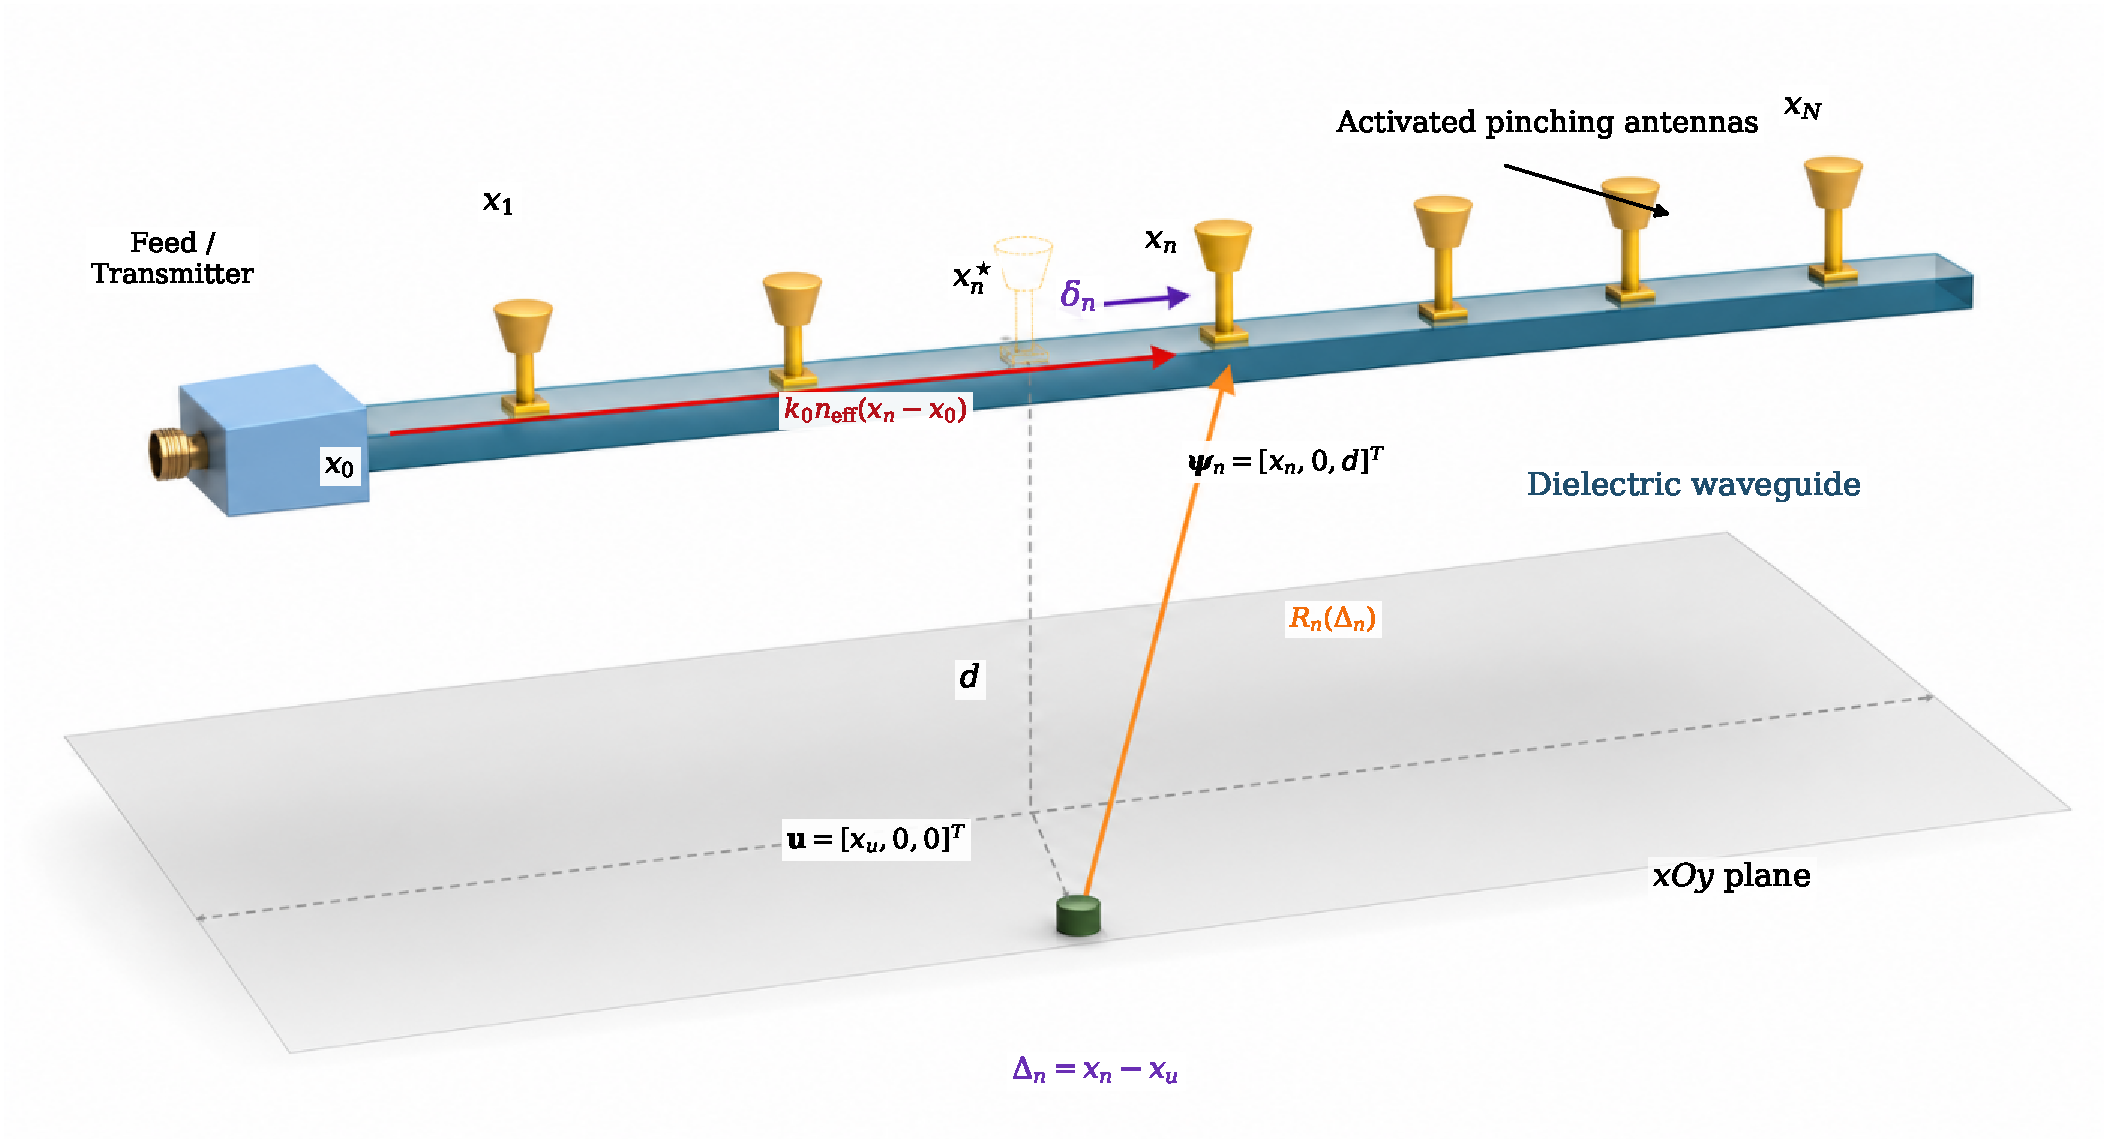
\includegraphics[width=0.78\textwidth]{figures/fig_pass_system_model_3d_minimal.pdf}
\caption[Three-dimensional PASS view]{Three-dimensional view of the same PASS system model. This visual is included to make the waveguide, activated pinching antennas, user location, and propagation paths easier to read; the analytical model remains the two-dimensional symmetric geometry defined in Section~2.}
\label{fig:pass_system_model_3d}
\end{figure}

\subsection{Project Scope and Relation to the Base PASS Paper}

This final-year project builds directly on the array-gain formulation of PASS in \cite{ouyang2025array}. The starting point is the single-user symmetric geometry used in that paper, together with its constructive phase-alignment viewpoint. The base literature shows how to design a nominal placement so that the phasors add coherently under ideal pinching positions. This project keeps that nominal starting point fixed and studies a new problem: once the constructive phase-aligned feasible placement is perturbed by bounded or random position errors, which degradation mechanisms dominate, what part of the degradation can be bounded analytically, and how much of the remaining behavior can still be explained by a small set of interpretable quantities?

The distinction between inherited theory and the project's own contribution remains explicit throughout the report. The system geometry, free-space path, waveguide phase, and normalized array-gain objective that define PASS are drawn from \cite{ouyang2025array}. The constructive aligned placement adopted here reframes the phase-alignment concept as a wavelength-snapped design that satisfies spacing constraints—this reformulation constitutes the project-level contribution. With this feasible nominal placement in hand, the robustness analysis advances through four interconnected steps. A position-dependent phase sensitivity is derived to quantify how strongly each activated pinching position affects the coherent sum. Under bounded errors, a deterministic lower bound follows, valid within a first-order small-error regime. To account for the dominant error mechanism beyond that narrow bound, a weighted phase-variance perspective is introduced, explaining why a left–right split perturbation proves empirically damaging whereas a common signed shift remains almost harmless. The same phase-variance object is then extended to stochastic error models, producing a covariance-based second-order predictor that covers i.i.d., common-bias, and correlated perturbations.

Choosing to fix a single constructive nominal design rather than re-optimizing the placement under every uncertainty law is a deliberate methodological decision. It centers the investigation on deeply understanding one reproducible design instead of superficially comparing many partly incomparable designs. Such a strategy fits a long-form graduation report especially well: it makes the chain of evidence easier to follow, since the same geometry, nominal reference, and sensitivity profile persist from the model definition through the deterministic bound and the stochastic predictor to the baseline interpretation.


\subsection{Literature Survey}

The PASS literature can be read as progressing from architecture definition to nominal design and then to broader application scenarios. The foundational PASS papers establish the waveguide-and-pinching architecture and explain why movable activation points create a new form of geometry control in wireless systems \cite{fukuda2022pinching,ding2025perspective}. Building on that model, later studies examine what can be achieved when the pinching positions are assumed ideal: constructive array-gain analysis in the single-user setting \cite{ouyang2025array}, downlink rate-oriented design \cite{xu2025downlink}, NOMA-oriented activation strategies \cite{wang2025noma}, and uplink fairness formulations \cite{tegos2025uplink}. Recent tutorial and outlook papers further widen the scope toward system-level interpretation and sensing-oriented extensions \cite{ding2025isac,liu2026tutorial}. Taken together, these papers make the nominal potential of PASS increasingly clear, but they still leave the robustness of those nominal placements largely untreated.

What these PASS papers share is an ideal-actuation viewpoint. The technical questions differ, but once a placement or activation set is selected, the resulting coordinates are effectively treated as exact. That assumption is reasonable for demonstrating nominal capability, but it leaves two important questions open. First, it does not reveal whether constructive gain is naturally tolerant or intrinsically fragile. Second, it does not indicate which perturbation structures should be regarded as the relevant stress tests for PASS: independent per-element offsets, coherent drifts, or spatially correlated errors. The present report addresses those questions directly and uses them to separate deterministic, empirical, and stochastic statements later in the manuscript.

The broader flexible-antenna literature is also essential for positioning this project. Fluid antennas and movable antennas show that antenna geometry can be treated as a design variable rather than as a fixed hardware constraint \cite{wong2021fluid,zhu2024movable,new2025tutorial,zhu2025tutorialma}. This literature is useful in two ways. First, it provides the wider communications motivation for studying geometry adaptation in near-field and large-aperture regimes. Second, it clarifies the modeling rhythm that is now standard in this area: specify the geometry, state the mobility or placement constraint, define the channel law, and then optimize the performance objective induced by that controllable geometry. Even so, PASS cannot be reduced to a generic flexible-antenna model, because its phase law contains not only the spherical-wave term but also the guided-wave accumulation along the dielectric waveguide. That additional term is central to both constructive alignment and the position-sensitivity issue studied here.

The closest comparison class comes from recent robustness studies under geometry uncertainty. Near-field and large-aperture communications already show that location-dependent phase and spherical-wave propagation can make geometry errors much more consequential than in far-field beamforming \cite{ouyang2024primer}. More specifically, recent movable-antenna studies have started to quantify the effect of position errors in near-field beamforming and flexible-array optimization \cite{su2025positionerror,yang2026nearfield}. These papers are important because they show that robustness cannot be treated as a minor implementation detail once antenna location becomes part of the design space. However, their uncertainty mechanism is still tied to free-space geometry control. The PASS setting adds the refractive-index-weighted waveguide term, so the relevant local sensitivity and the most damaging perturbation patterns need not match the movable-antenna case.

For that reason, the present survey is organized by technical axis rather than by author chronology. The key categories are PASS foundations and tutorials, PASS nominal design and application papers, the broader flexible-antenna context, and geometry-uncertainty robustness studies. Organizing the literature in this way suits a longer report, because it surfaces shared and missing assumptions simultaneously. In particular, it shows that the gap is not the broad statement that robustness has not been studied anywhere, but the narrower, more defensible claim that the cited literature does not adequately explain PASS-specific robustness for constructive phase-aligned placement.

These three strands of literature thus reveal a clear gap. The PASS community possesses well-developed nominal models and growing application coverage, and the wider flexible-antenna community has begun to confront geometry uncertainty; yet the cited PASS works still lack a focused explanation of how constructive phase-aligned PASS placement degrades under bounded and stochastic pinching-position errors. To fill this gap, the report limits itself to the single-user symmetric geometry of \cite{ouyang2025array}, a single feasible nominal design, and an investigation of how deterministic bounds, interpretable adversarial patterns, and stochastic covariance jointly explain robustness—a deliberate narrowness that separates deterministic small-error arguments from empirical observations instead of blending them into a broader, weaker claim.

By condensing the literature architecture into the four categories that matter here, Table~\ref{tab:literature_map} serves both as a scannable survey chapter and as a map that situates the project precisely within existing PASS and flexible-antenna work.

\begin{table}[H]
\centering
\small
\caption{Category-based literature map and the specific gap addressed in this report.}
\label{tab:literature_map}
\begin{tabularx}{\textwidth}{>{\raggedright\arraybackslash}p{0.22\textwidth} >{\raggedright\arraybackslash}p{0.28\textwidth} >{\raggedright\arraybackslash}p{0.18\textwidth} >{\raggedright\arraybackslash}X}
\toprule
Category & Representative focus & Key references & Relevance to this report \\
\midrule
PASS foundations and architecture & Waveguide-enabled activation, system concept, and broad PASS framing & \cite{fukuda2022pinching,ding2025perspective,liu2026tutorial} & Establishes the PASS model class, but does not analyze robustness under pinching-position errors. \\
PASS nominal design and applications & Nominal constructive gain, downlink rate design, NOMA activation, uplink fairness, sensing extensions & \cite{ouyang2025array,xu2025downlink,wang2025noma,tegos2025uplink,ding2025isac} & Provides the nominal starting point and application context inherited here. \\
Flexible-antenna context & Fluid and movable antennas as geometry-controlled communication systems & \cite{wong2021fluid,zhu2024movable,new2025tutorial,zhu2025tutorialma} & Explains why geometry control matters, but does not capture the PASS-specific guided-wave phase term. \\
Position uncertainty and near-field robustness & Geometry-error sensitivity in near-field or movable-antenna beamforming & \cite{ouyang2024primer,su2025positionerror,yang2026nearfield} & Gives the closest robustness analogue and motivates a dedicated PASS error study. \\
\bottomrule
\end{tabularx}
\end{table}

In compact form, the inherited material from prior PASS work is the system geometry, channel law, and nominal phase-alignment motivation. The new material in this project is the feasible constructive placement reformulation, the bounded- and stochastic-error robustness analysis, and the narrow same-aperture baseline comparison. What is not claimed is any exact continuous-box worst-case solution or any globally optimal PASS placement result.

\subsection{Objectives, Contributions, and Non-Claims}

The technical gap addressed here can be stated precisely. Existing PASS literature explains how constructive phase alignment improves nominal coherent addition \cite{ding2025perspective,ouyang2025array}. What is still missing is a position-error theory that is (1) local enough to permit explicit derivations and validity conditions, (2) sufficiently interpretable to explain why distinct perturbation patterns produce qualitatively different behaviour, (3) broad enough to bridge deterministic bounded-error models with stochastic error covariance models, and (4) conservative enough to avoid over-claiming global optimality or universal design rules.

This report addresses that gap for one coherent fixed configuration. The simulation setup is $N = 16$, $d = \SI{3}{m}$, $f_c = \SI{28}{GHz}$, $n_{\mathrm{eff}} = 1.44$, and $\Delta_p = 0.5\lambda$. The constructive phase-aligned placement generated from this setup is then analyzed under bounded box errors, Monte Carlo perturbations, and several placement baselines. The result is a complete evidence chain from system model to design construction, perturbation theory, numerical validation, and claim-disciplined conclusions.

The main contributions of the report are summarized below.

\begin{itemize}
\item A PASS robustness formulation is built directly on the array-gain model of \cite{ouyang2025array}, but rewritten around the constructive phase-aligned feasible placement generated under spacing constraints. This makes the nominal design explicit and reproducible.
\item A position-dependent phase sensitivity $\xi_n$ and a deterministic lower bound are derived for bounded position errors. For the studied design, the first-order deterministic validity threshold is $\epsilon/\lambda = 0.1713$, and within that region the lower bound tracks the box-best-found degradation curve almost exactly.
\item A weighted phase-variance interpretation is developed to unify deterministic and stochastic robustness behavior. The same object explains why an empirical left-right split-mode perturbation nearly matches the box-best-found adversary before the first null, while common-bias motion produces almost no degradation.
\item A covariance-based stochastic predictor is derived and validated for iid uniform, common-bias, and correlated Gaussian error models. This gives a compact explanation of why statistically smooth perturbations are much less damaging than independent ones with the same marginal variance.
\item A narrow comparative design statement is established: in the tested same-aperture comparison, the constructive aligned placement is stronger than a naive uniform-aperture placement, especially in box-best-found robustness, but it is not the best tested design because a best-found nominal-gain comparator outperforms it on every reported metric.
\end{itemize}

Taken together, these contributions form a single, continuous argument—not five independent points. The constructive placement provides the reference geometry; the deterministic analysis establishes the bounds of what can be justified in the small-error regime. The split-mode mechanism explains the dominant harmful bounded perturbation up to the first null, the covariance predictor captures the ordering of the stochastic curves, and the baseline section measures the design value retained by the constructive rule relative to straightforward same-aperture alternatives. The logic constructed at this stage is what later allows the conclusions to remain conservative without becoming vague.

The report also explicitly disclaims several assertions. It does not claim a globally certified continuous-box optimum for the worst-case problem, nor that the split-mode pattern is the exact optimizer of the bounded-box adversary. No assertion of general design optimality is made over arbitrary PASS placements, antenna counts, or geometries. Further, the stochastic predictor is not extended beyond the tested small-error range or the constructive design examined here. These disclaimers are integral to the argument, not incidental; they shape how the evidence is presented.

\subsection{Report Organization}

We structure the rest of the paper accordingly. Section~2 outlines the framework, covering the inherited PASS model, constructive nominal placement, the position-error formulation, a deterministic lower bound, the weighted phase-variance mechanism, and the numerical evaluation protocol. Section~3 reports the results of deterministic, stochastic, and baseline-comparison analyses. In Section~4, we analyze the mechanisms behind these results and disentangle the deterministic small-error guarantees from the empirical observations. Section~5 concludes with key takeaways and promising avenues for future research. The appendices provide the full derivations and secondary sensitivity analyses that support the main text.
